\documentclass[tikz]{standalone}
\usepackage{amsmath,amssymb}
\newcommand{\la}[1]{\boldsymbol{#1}}
\usepackage{pgf}
\usepackage{tikz}
\usetikzlibrary{arrows,automata}
\usepackage[latin1]{inputenc}
\begin{document}
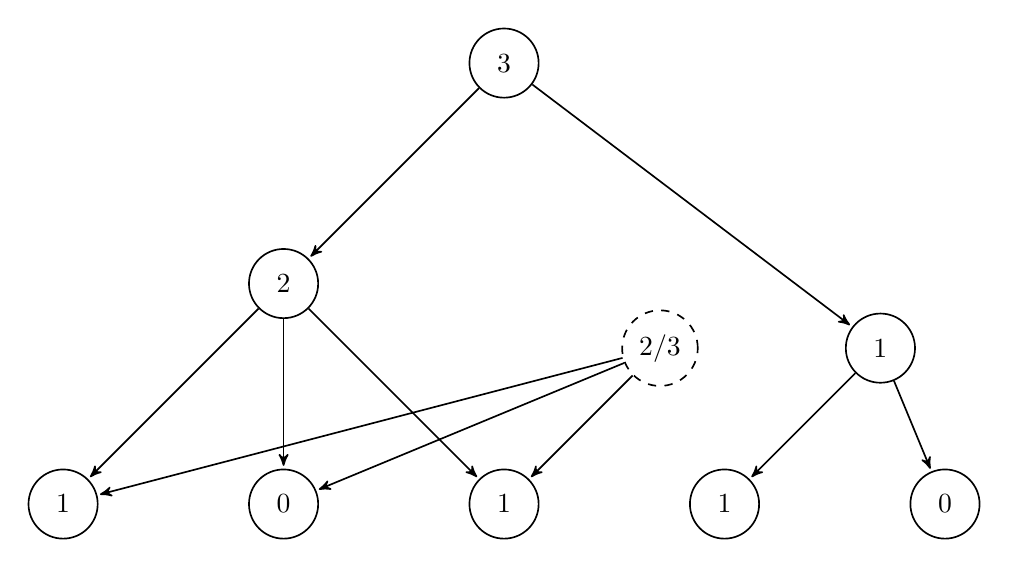
\begin{tikzpicture}[->,>=stealth',shorten >=1pt,auto,node distance=2.8cm,
                    semithick]

  \node[state]  (A)              {$1$};
  \node[state]  (B) [right of=A] {$0$};
  \node[state]  (C) [right of=B] {$1$};
  \node[state]  (D) [right of=C] {$1$};
  \node[state]  (E) [right of=D] {$0$};
 
  \node[state]  (F) [above of=B] {$2$};
  \path (F) edge (A); 
  \path (F) edge (B);
  \path (F) edge (C);

  \node[state] (G) [above right of = D] {$1$};
  \path (G) edge (D);
  \path (G) edge (E);

  \node[state] (H) [right of = C, above of = F] {$3$};
  \path(H) edge (F);
  \path(H) edge (G);

  \node[state, dashed] (I) [above right of = C] {$2/3$};
  \path (I) edge (A);
  \path (I) edge (B);
  \path (I) edge (C);


\end{tikzpicture}

\end{document}
